% !TEX program = pdflatex
% !BIB program = biber

\documentclass{article}

\usepackage{arxiv}
\usepackage{algorithm,algorithmic}
\usepackage{bm}
\usepackage{amsmath}
\usepackage{amssymb}
% \usepackage{mathptmx} 
% theorems
\usepackage{amsthm}

\usepackage[utf8]{inputenc} % allow utf-8 input
\usepackage[T1]{fontenc}    % use 8-bit T1 fonts
\usepackage{hyperref}       % hyperlinks
\usepackage{url}            % simple URL typesetting
\usepackage{booktabs}       % professional-quality tables
\usepackage{amsfonts}       % blackboard math symbols
\usepackage{nicefrac}       % compact symbols for 1/2, etc.
\usepackage{microtype}      % microtypography
\usepackage{cleveref}       % smart cross-referencing
\usepackage{lipsum}         % Can be removed after putting your text content
\usepackage{graphicx}
% \usepackage[numeric]{natbib}
\usepackage[backend=bibtex,style=ieee]{biblatex}
\bibliography{references}  
\DeclareFieldFormat{url}{}
\DeclareFieldFormat{urldate}{}
\usepackage{doi}

\title{Guaranteed Parallel Co-clustering on Big Matrices}

% Here you can change the date presented in the paper title
%\date{September 9, 1985}
% Or remove it
%\date{}

\newif\ifuniqueAffiliation
% Uncomment to use multiple affiliations variant of author block 
\uniqueAffiliationtrue

\ifuniqueAffiliation % Standard variant of author block
\author{ 
	% \href{https://orcid.org/0000-0000-0000-0000}{
\includegraphics[scale=0.06]{orcid.pdf}\hspace{1mm}David S.~Hippocampus}\thanks{Use footnote for providing further
	% 	information about author (webpage, alternative
	% 	address)---\emph{not} for acknowledging funding agencies.} \\
	% Department of Computer Science\\
	% Cranberry-Lemon University\\
	% Pittsburgh, PA 15213 \\
	% \texttt{hippo@cs.cranberry-lemon.edu} \\
	% %% examples of more authors
	% \And
	% \href{https://orcid.org/0000-0000-0000-0000}{
\includegraphics[scale=0.06]{orcid.pdf}\hspace{1mm}Elias D.~Striatum} \\
	% Department of Electrical Engineering\\
	% Mount-Sheikh University\\
	% Santa Narimana, Levand \\
	% \texttt{stariate@ee.mount-sheikh.edu} \\
	% \AND
	% Coauthor \\
	% Affiliation \\
	% Address \\
	% \texttt{email} \\
	% \And
	% Coauthor \\
	% Affiliation \\
	% Address \\
	% \texttt{email} \\
	% \And
	% Coauthor \\
	% Affiliation \\
	% Address \\
	% \texttt{email} \\
}
\else
% Multiple affiliations variant of author block
\usepackage{authblk}
\renewcommand\Authfont{\bfseries}
\setlength{\affilsep}{0em}
% box is needed for correct spacing with authblk
\newbox{\orcid}\sbox{\orcid}{
\includegraphics[scale=0.06]{orcid.pdf}} 
\author[1]{%
	\href{https://orcid.org/0000-0000-0000-0000}{\usebox{\orcid}\hspace{1mm}David S.~Hippocampus\thanks{\texttt{hippo@cs.cranberry-lemon.edu}}}%
}
\author[1,2]{%
	\href{https://orcid.org/0000-0000-0000-0000}{\usebox{\orcid}\hspace{1mm}Elias D.~Striatum\thanks{\texttt{stariate@ee.mount-sheikh.edu}}}%
}
\affil[1]{Department of Computer Science, Cranberry-Lemon University, Pittsburgh, PA 15213}
\affil[2]{Department of Electrical Engineering, Mount-Sheikh University, Santa Narimana, Levand}
\fi

% Uncomment to override  the `A preprint' in the header
%\renewcommand{\headeright}{Technical Report}
%\renewcommand{\undertitle}{Technical Report}
\renewcommand{\shorttitle}{\textit{arXiv} Template}

% new command
%% define \cite{} to represent ~\autocite{}
\renewcommand{\cite}[1]{~\autocite{#1}}

%%% Add PDF metadata to help others organize their library
%%% Once the PDF is generated, you can check the metadata with
%%% ```pdfinfo template.pdf```
\hypersetup{
pdftitle={A template for the arxiv style},
pdfsubject={q-bio.NC, q-bio.QM},
pdfauthor={David S.~Hippocampus, Elias D.~Striatum},
pdfkeywords={First keyword, Second keyword, More},
}

\begin{document}
\maketitle

\begin{abstract}
	\lipsum[1]
\end{abstract}


% keywords can be removed
\keywords{First keyword \and Second keyword \and More}


%%%
% File: /latex/big-cocluster-paper/sections/introduction.tex
% Created Date: Thursday, July 11th 2024
% Author: Zihan
% -----
% Last Modified: Sunday, 14th July 2024 9:44:18 pm
% Modified By: the developer formerly known as Zihan at <wzh4464@gmail.com>
% -----
% HISTORY:
% Date      		By   	Comments
% ----------		------	---------------------------------------------------------
%%%

\section{Introduction}
Artificial Intelligence is a rapidly advancing technology facilitating complex data analysis, pattern recognition, and decision-making processes. Clustering, a fundamental unsupervised learning technique, groups data points based on shared features, aiding in interpreting complex data structures. However, traditional clustering algorithms \cite{zhang2023AdaptiveGraphConvolution, wu2023EffectiveClusteringStructured} treat all features of data uniformly and solely cluster either rows (samples) or columns (features),  as shown in Figure \ref{fig:cluster}. They oversimplified interpretations and overlooked critical context-specific relationships within the data, especially when dealing with large, high-dimensional datasets \cite{chen2023FastFlexibleBipartite, zhao2023MultiviewCoclusteringMultisimilarity, kumar2023CoclusteringBasedMethods}.

\textit{Co-clustering} \cite{kluger2003SpectralBiclusteringMicroarray, yan2017CoclusteringMultidimensionalBig} is a technique that groups rows (samples) and columns (features) simultaneously, as shown in Figure \ref{fig:cocluster}. It can reveal complex correlations between two different data types and is transformative in scenarios where the relationships between rows and columns are as important as the individual entities themselves. For example, in bioinformatics, co-clustering could identify gene-related patterns leading to biological insights by concurrently analyzing genes and conditions \cite{higham2007SpectralClusteringIts, kluger2003SpectralBiclusteringMicroarray, zhao2012BiclusteringAnalysisPattern}. In recommendation systems, co-clustering can simultaneously discover more fine-grained relationships between users and projects \cite{dhillon2007WeightedGraphCuts, chen2023ParallelNonNegativeMatrix}. Co-clustering extends traditional clustering methods, enhancing accuracy in pattern detection and broadening the scope of analyses.

% insert cocomparison.png here
\begin{figure}[htbp]
    \centering
    \begin{subfigure}[b]{0.22\textwidth}
        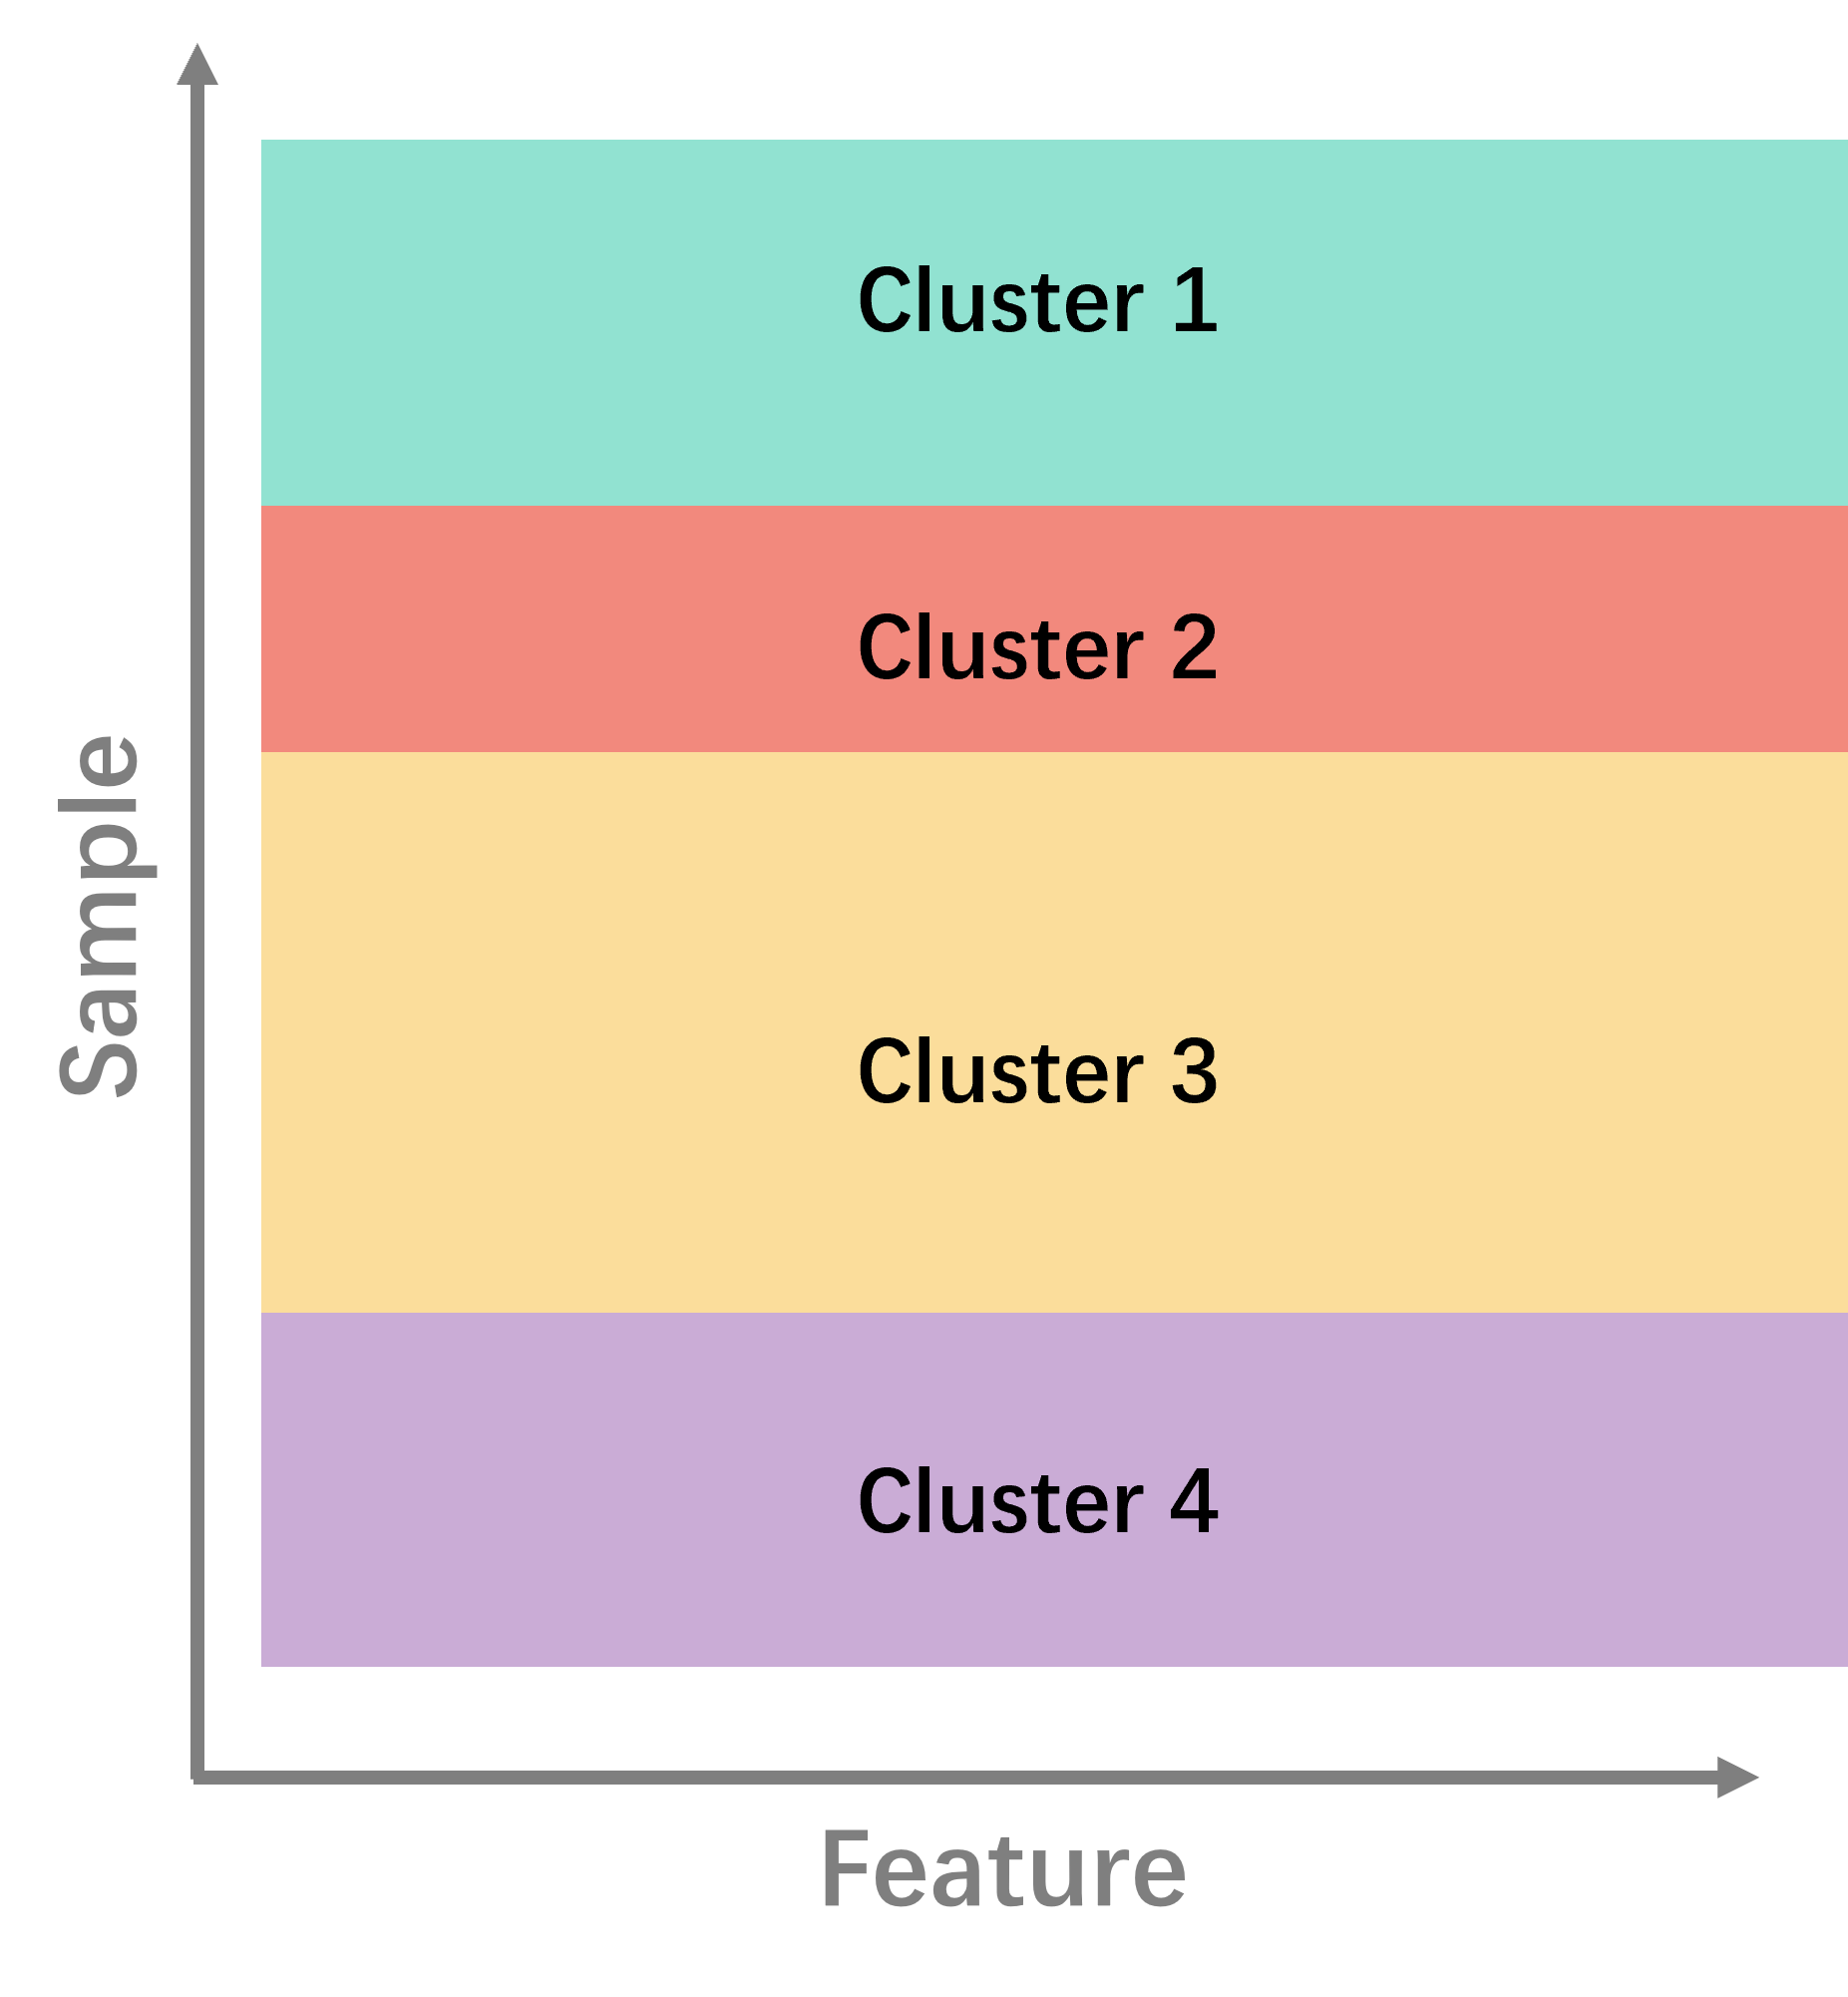
\includegraphics[width=\linewidth]{cluster.png}
        \caption{Clustering}
        \label{fig:cluster}
    \end{subfigure}
    \hfill
    \begin{subfigure}[b]{0.22\textwidth}
        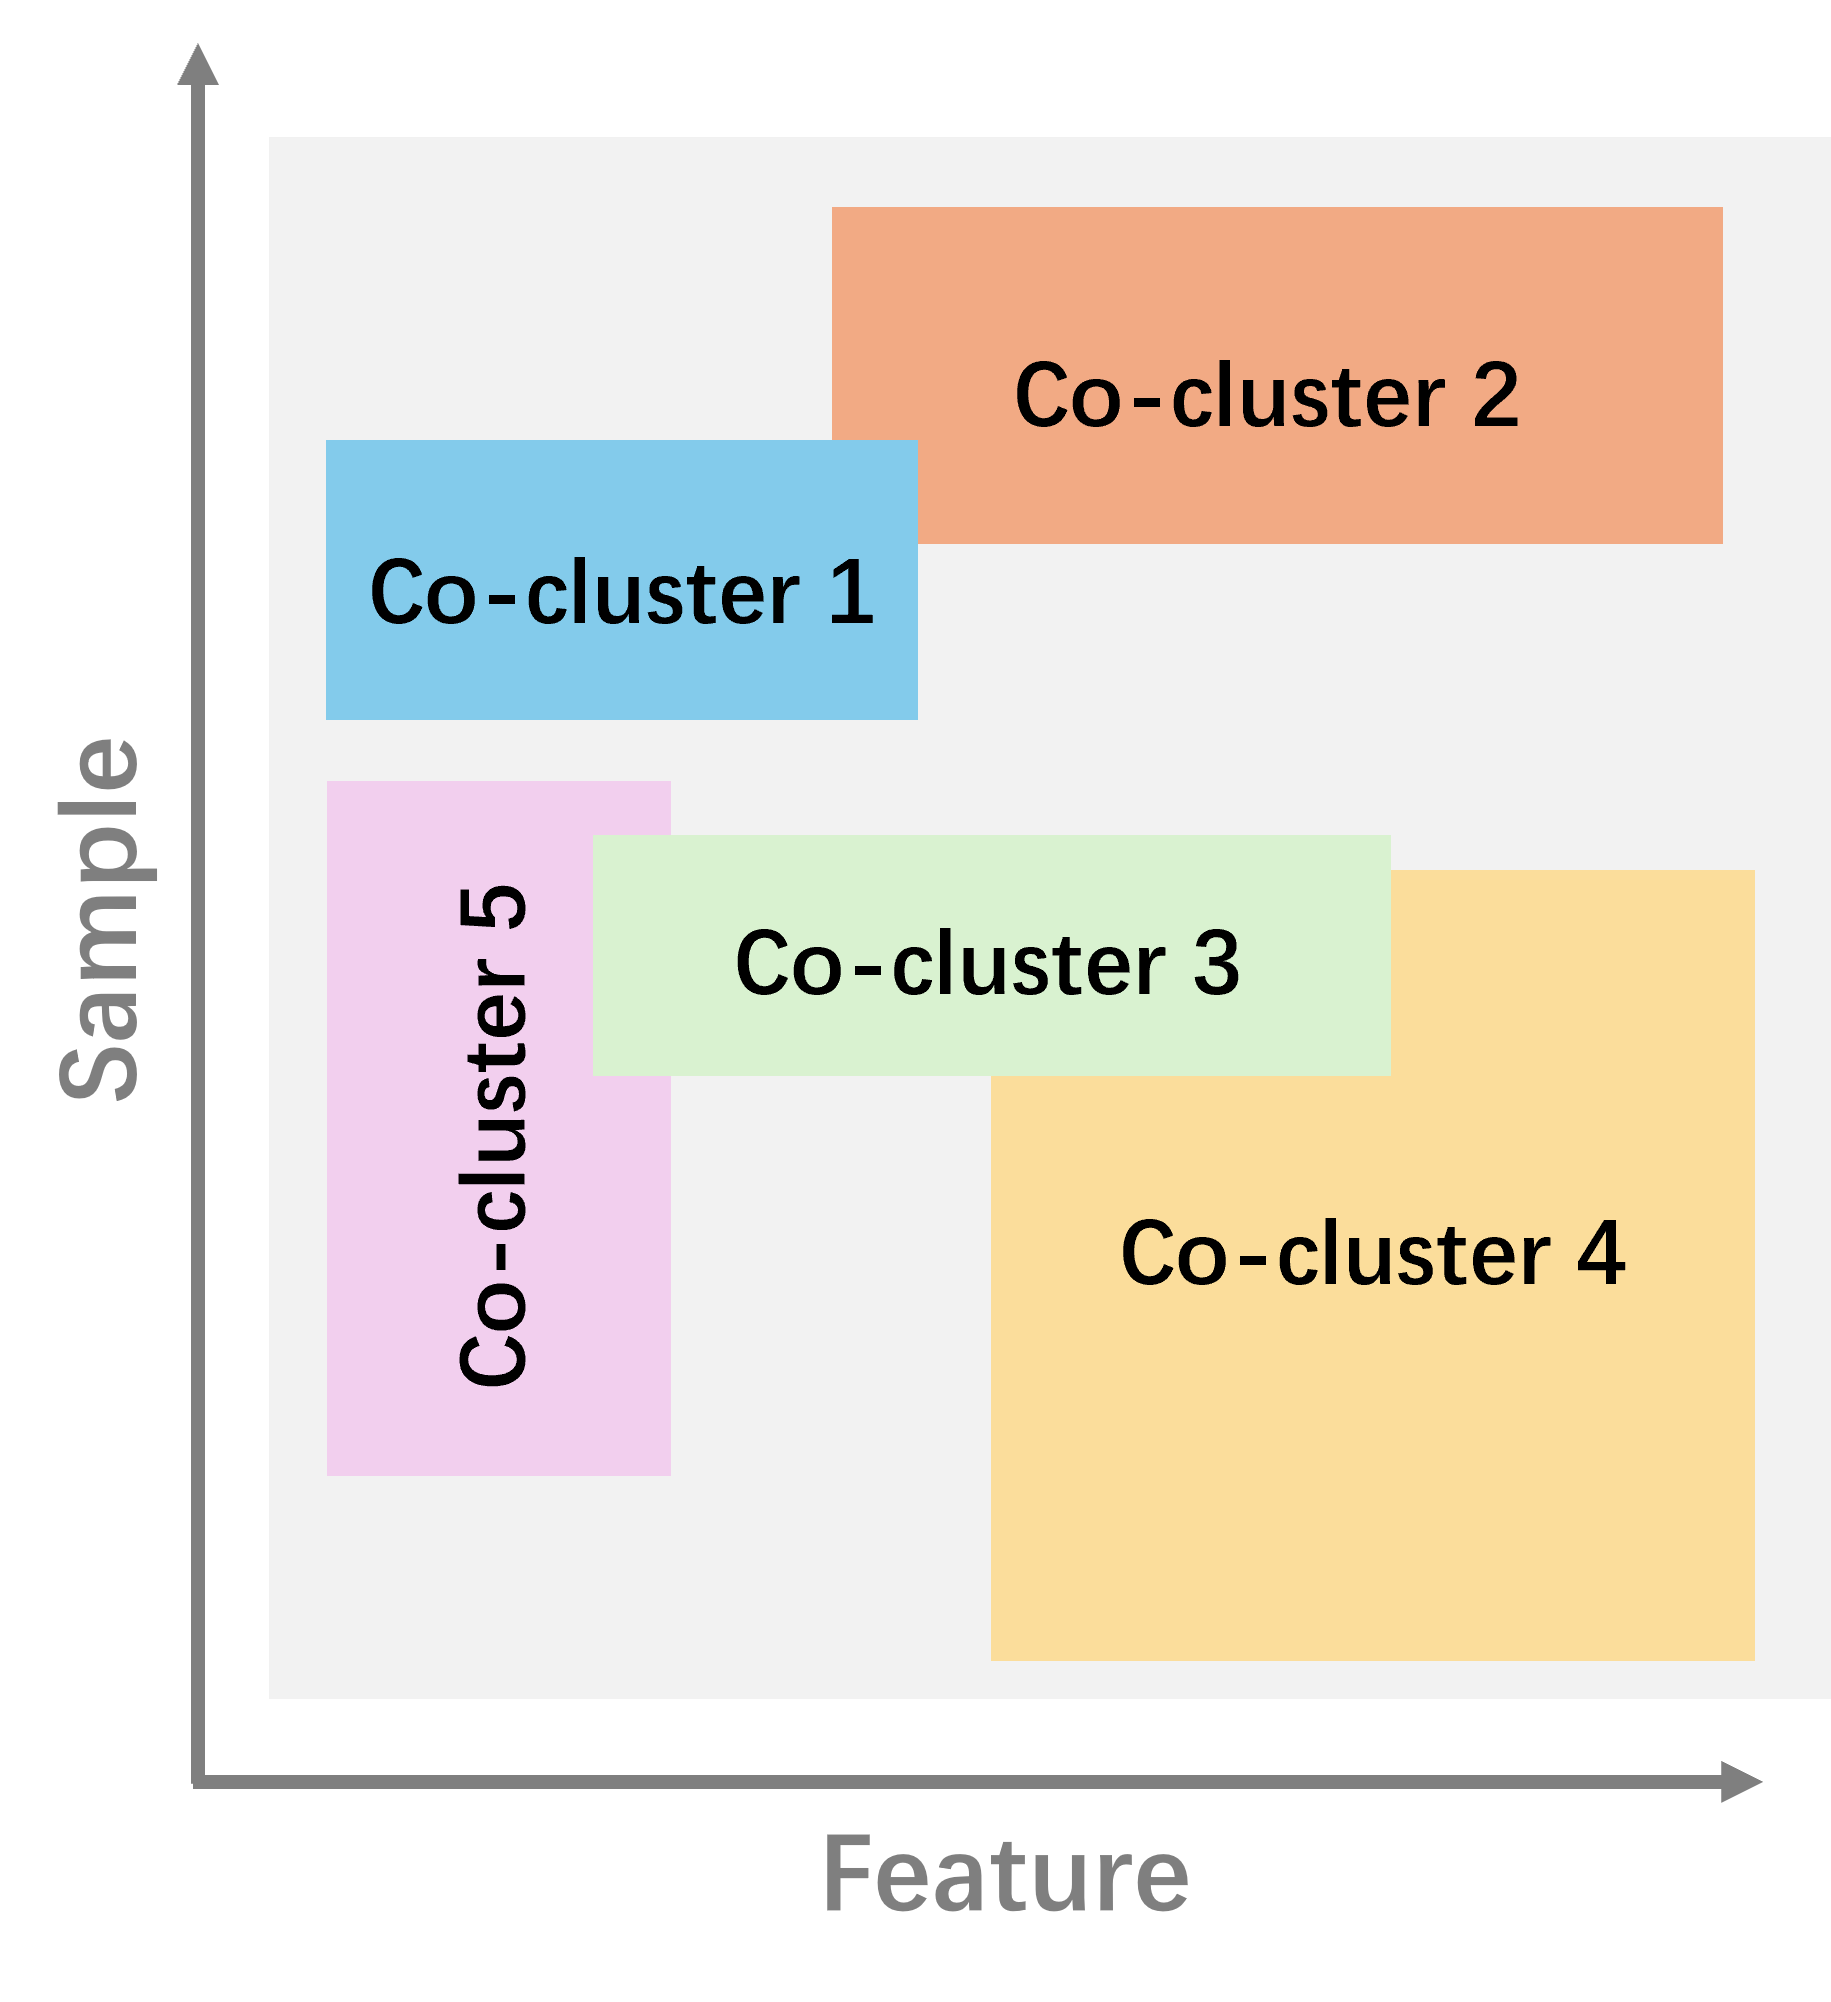
\includegraphics[width=\linewidth]{coc.png}
        \caption{Co-clustering}
        \label{fig:cocluster}
    \end{subfigure}
    \caption{An illustration of the differences between (a) Clustering and (b) Co-clustering \cite{yan2017CoclusteringMultidimensionalBig}.}
    \label{fig:cocomparison}
\end{figure}

Despite its potential, scaling co-clustering to large datasets poses significant challenges:

\begin{itemize}
    \item{\textbf{High Computational Complexity.}} Co-clustering analyzes relationships both within and across the rows and columns of a dataset simultaneously. This dual-focus analysis requires evaluating a vast number of potential relationships, particularly as the dimensions of the data increase. The complexity can grow exponentially with the size of the data because the algorithm must process every possible combination of rows and columns to identify meaningful clusters \cite{hansen2011NonparametricCoclusteringLarge}.
    \item{\textbf{Significant Communication Overhead.}} Even when methods such as data partitioning are used to handle large-scale data, each partition may independently analyze a subset of the data. However, to optimize the clustering results globally, these partitions need to exchange intermediate results frequently. This requirement is inherent to iterative optimization techniques used in co-clustering, where each iteration aims to refine the clusters based on new data insights, necessitating continuous updates across the network. Such extensive communication can become a bottleneck, significantly slowing down the overall processing speed.
    \item{\textbf{Dependency on Sparse Matrices.}} Several traditional co-clustering algorithms are designed to perform best with sparse matrices \cite{pan2008CRDFastCoclusteringa}. However, in many real-world applications, data matrices are often dense, meaning most elements are non-zero. Such scenarios present a significant challenge for standard co-clustering algorithms, as they must handle a larger volume of data without the computational shortcuts available with sparse matrices.
\end{itemize}

To address the inherent challenges associated with existing co-clustering methods, we propose a novel and scalable Adaptive Hierarchical Partitioning and Merging for Scalable Co-Clustering (\textbf{AHPM}) framework designed for large-scale datasets. First,  we propose a large matrix partitioning algorithm that divides the original data matrix into smaller submatrices. This partitioning facilitates parallel processing of co-clustering tasks across submatrices, significantly reducing both processing time and computational and storage demands for each processing unit. We also design a probabilistic model to determine the optimal number and configuration of these submatrices to ensure comprehensive data coverage.
Second, we develop a hierarchical co-cluster merging algorithm that iteratively combines the co-clusters from these submatrices. This process enhances the accuracy and reliability of the final co-clustering results and ensures robust and consistent clustering performance, particularly addressing issues of heterogeneity and model uncertainty.

The contributions of this paper are summarized as follows:
\begin{enumerate}
    \item \textbf{Large Matrix Partitioning Algorithm:}
          We propose a novel matrix partitioning algorithm that enables parallel co-clustering by dividing a large matrix into optimally configured submatrices. This design is supported by a probabilistic model that calculates the optimal number and order of submatrices, balancing computational efficiency with the detection of relevant co-clusters.
    \item \textbf{Hierarchical Co-cluster Merging Algorithm:}
          We design a hierarchical co-cluster merging algorithm that combines co-clusters from submatrices, ensuring the completion of the co-clustering process within a pre-fixed number of iterations. This algorithm significantly enhances the robustness and reliability of the co-clustering process, effectively addressing model uncertainty.
    \item \textbf{Experimental Valuation:}
          We evaluate the effectiveness and efficiency of our method across a wide range of scenarios with large, complex data. Experimental results show an approximate 83\% decrease for dense matrices and up to 30\% for sparse matrices.
\end{enumerate}

The rest of this paper is organized as: Section \ref{sec:related_work} reviews related works; Section \ref{sec:formula} presents the problem formulation; Section \ref{sec:method} describes our AHPM method; Section \ref{sec:experiment} reports experimental results; and Section \ref{sec:conclude} concludes the paper.


% !TeX root = main.tex

%%%
% File: /latex/big-cocluster-paper/related_work.tex
% Created Date: Monday, December 18th, 2023
% Author: Zihan
% -----
% Last Modified: Monday, 18th December 2023 5:23:36 pm
% Modified By: the developer formerly known as Zihan at <wzh4464@gmail.com>
% -----
% HISTORY:
% Date      		By   	Comments
% ----------		------	---------------------------------------------------------
% 19-12-2023		Zihan	Complete the first draft of Related Work
%%%

\section{Related work}
\subsection{Neural Network models}
Dong \textit{et al.}\cite{dongkuanxu2019DeepCoClustering} proposed DeepCC, the first deep-learning model for co-clustering. DeepCC employs deep autoencoders and Gaussian Mixture Models to simultaneously cluster instances and features in an end-to-end fashion. A mutual information loss connects the joint instance and feature representation learning. {\color{blue} However, DeepCC is limited to static data, because it does not support incremental updates. Besides, DeepCC does not scale well to large datasets due to its high computational complexity.}
Besides, DeepCC does not scale well to large datasets due to its high computational complexity.}

If others said these cons, you need to add ref to show not you diss DeepCC}. 

\subsection{Matrix factorization}
%TODO: Overview: \cite{lin2019OverviewCoClusteringMatrix}
Kluger et al. \cite{kluger2003SpectralBiclusteringMicroarray} developed a spectral biclustering method that utilizes Singular Value Decomposition (SVD) to find checkerboard structures corresponding to genes differentially expressed across subsets of conditions in gene expression data.   

A pivotal shift in co-clustering methodology emerged with the adoption of matrix factorization techniques. This approach, fundamentally different from traditional clustering methods, factors the data matrix into multiple matrices, revealing underlying patterns and associations between rows and columns. The introduction of Non-negative Matrix Factorization (NMF) in co-clustering marked a significant advancement. By decomposing the sample-feature matrix into separate matrices for samples and features, NMF-based co-clustering techniques, such as the orthogonal NMTF by Ding \textit{et al.} \cite{ding2006OrthogonalNonnegativeMatrix}, provided a more interpretable and efficient way to identify clusters. 

Following this, various enhancements and extensions to matrix factorization in co-clustering were proposed. Methods like Fast Non-negative Matrix Tri-factorization (FNMTF) \cite{wang2019DualHypergraphRegularized}and Bilateral k-means (BKM) \cite{junweihan2017BilateralKMeansAlgorithm} further refined the approach by introducing constraints and optimizations that improved computational speed and accuracy.  

The matrix factorization-based co-clustering has not only been limited to static data analysis but also extended to dynamic scenarios. This adaptation is evident in applications like real-time collaborative filtering and online text mining, where the ability to update co-clusters incrementally becomes crucial \cite{daruru2009PervasiveParallelismData}.



% Now, to process big data, MTF is the most popular method. \cite{chen2023ParallelNonNegativeMatrix}

 {\color{blue} While matrix factorization techniques have shown promise for co-clustering large datasets, scaling to massive high-dimensional data remains an open challenge. } Chen et al. \cite{chen2023ParallelNonNegativeMatrix} proposed a parallel non-negative matrix tri-factorization method that distributes computation across multiple nodes to accelerate factorizations.  {\color{blue} However, such approaches still struggle with web-scale data.}

Our proposed method takes a divide-and-conquer approach, directly partitioning the input matrix into smaller submatrices before co-clustering each one in parallel. This blocks the original high dimensionality to make co-clustering feasible. The separate results are then ensembled to produce final co-clusters. This represents a new paradigm tailored for big data that sidesteps computational barriers by transforming the problem space rather than relying solely on distributed computing optimizations.
% @Author: Zihan Wu
% @Date:   2024-04-20 21:21:00
% @Last Modified by:   Zihan Wu
% @Last Modified time: 2024-04-30 23:52:00
% sectionis/method.tex

\section{Mathematical Formulation and Problem Statement}\label{sec:formula}

\subsection{Mathematical Formulation of Co-clustering}
Co-clustering groups rows and columns of a data matrix $\mathbf{A} \in \mathbb{R}^{M \times N}$, where $M$ is the number of features and $N$ is the number of samples. Each element $a_{ij}$ represents the relationship between the $i$-th feature and the $j$-th sample. The goal is to partition $\mathbf{A}$ into $k$ row clusters and $d$ column clusters, creating $k \times d$ homogeneous submatrices $\mathbf{A}_{I, J}$.

When optimally reordered, $\mathbf{A}$ forms a block-diagonal structure where each block is a co-cluster with high internal similarity. Row and column labels are \( u \in \{1,\dots,k\}^M \) and \( v \in \{1,\dots,d\}^N \). Indicator matrices \( R \in \mathbb{R}^{M \times k} \) and \( C \in \mathbb{R}^{N \times d} \) assign rows and columns to clusters, ensuring unique assignments.

\subsection{Problem Statement}
This paper aims to develop a method to efficiently and accurately identify co-clusters $\mathbf{A}_{I, J}$ in large datasets. These co-clusters should exhibit uniformity, consistency, or specific patterns. Proper identification and categorization of these patterns are crucial for understanding complex data structures. Our method enhances co-clustering detection capabilities, improving efficiency and precision for large-scale data challenges.

\begin{table*}[h]
    \centering
    \begin{tabular}{c|p{10cm}}
        \hline
        \textbf{Symbol}        & \textbf{Description}                                                                                                           \\
        \hline
        $\mathbf{A}$           & Data matrix of dimensions $M \times N$, where $M$ is the number of rows (features) and $N$ is the number of columns (samples). \\
        $a_{ij}$               & Element at the $i$-th row and $j$-th column of matrix $\mathbf{A}$.                                                            \\
        $I, J$                 & Indices of rows and columns selected for co-clustering.                                                                        \\
        $\mathbf{A}_{I, J}$    & Submatrix containing the rows indexed by $I$ and columns by $J$.                                                               \\
        $k, d$                 & Number of row clusters and column clusters, respectively.                                                                      \\
        $R, C$                 & Indicator matrices for row and column cluster assignments.                                                                     \\
        $\phi_i, \psi_j$       & Block sizes in rows and columns, respectively.                                                                                 \\
        $s_i^{(k)}, t_j^{(k)}$ & Minimum row and column sizes of co-cluster $C_k$ in block $B_{(i,j)}$.                                                         \\
        $P(\omega_k)$          & Probability of failure to identify co-cluster $C_k$.                                                                           \\
        $T_p$                  & Number of sampling times or iterations in the probabilistic model.                                                             \\
        \hline
    \end{tabular}
    \caption{Notations used in the mathematical formulation of co-clustering}
    \label{tab:notations}
\end{table*}

\section{The Scalable Co-clustering Method}
\label{sec:method}
\subsection{Overview}

% insert workflow.png here
\begin{figure*}[htbp]
    \centering
    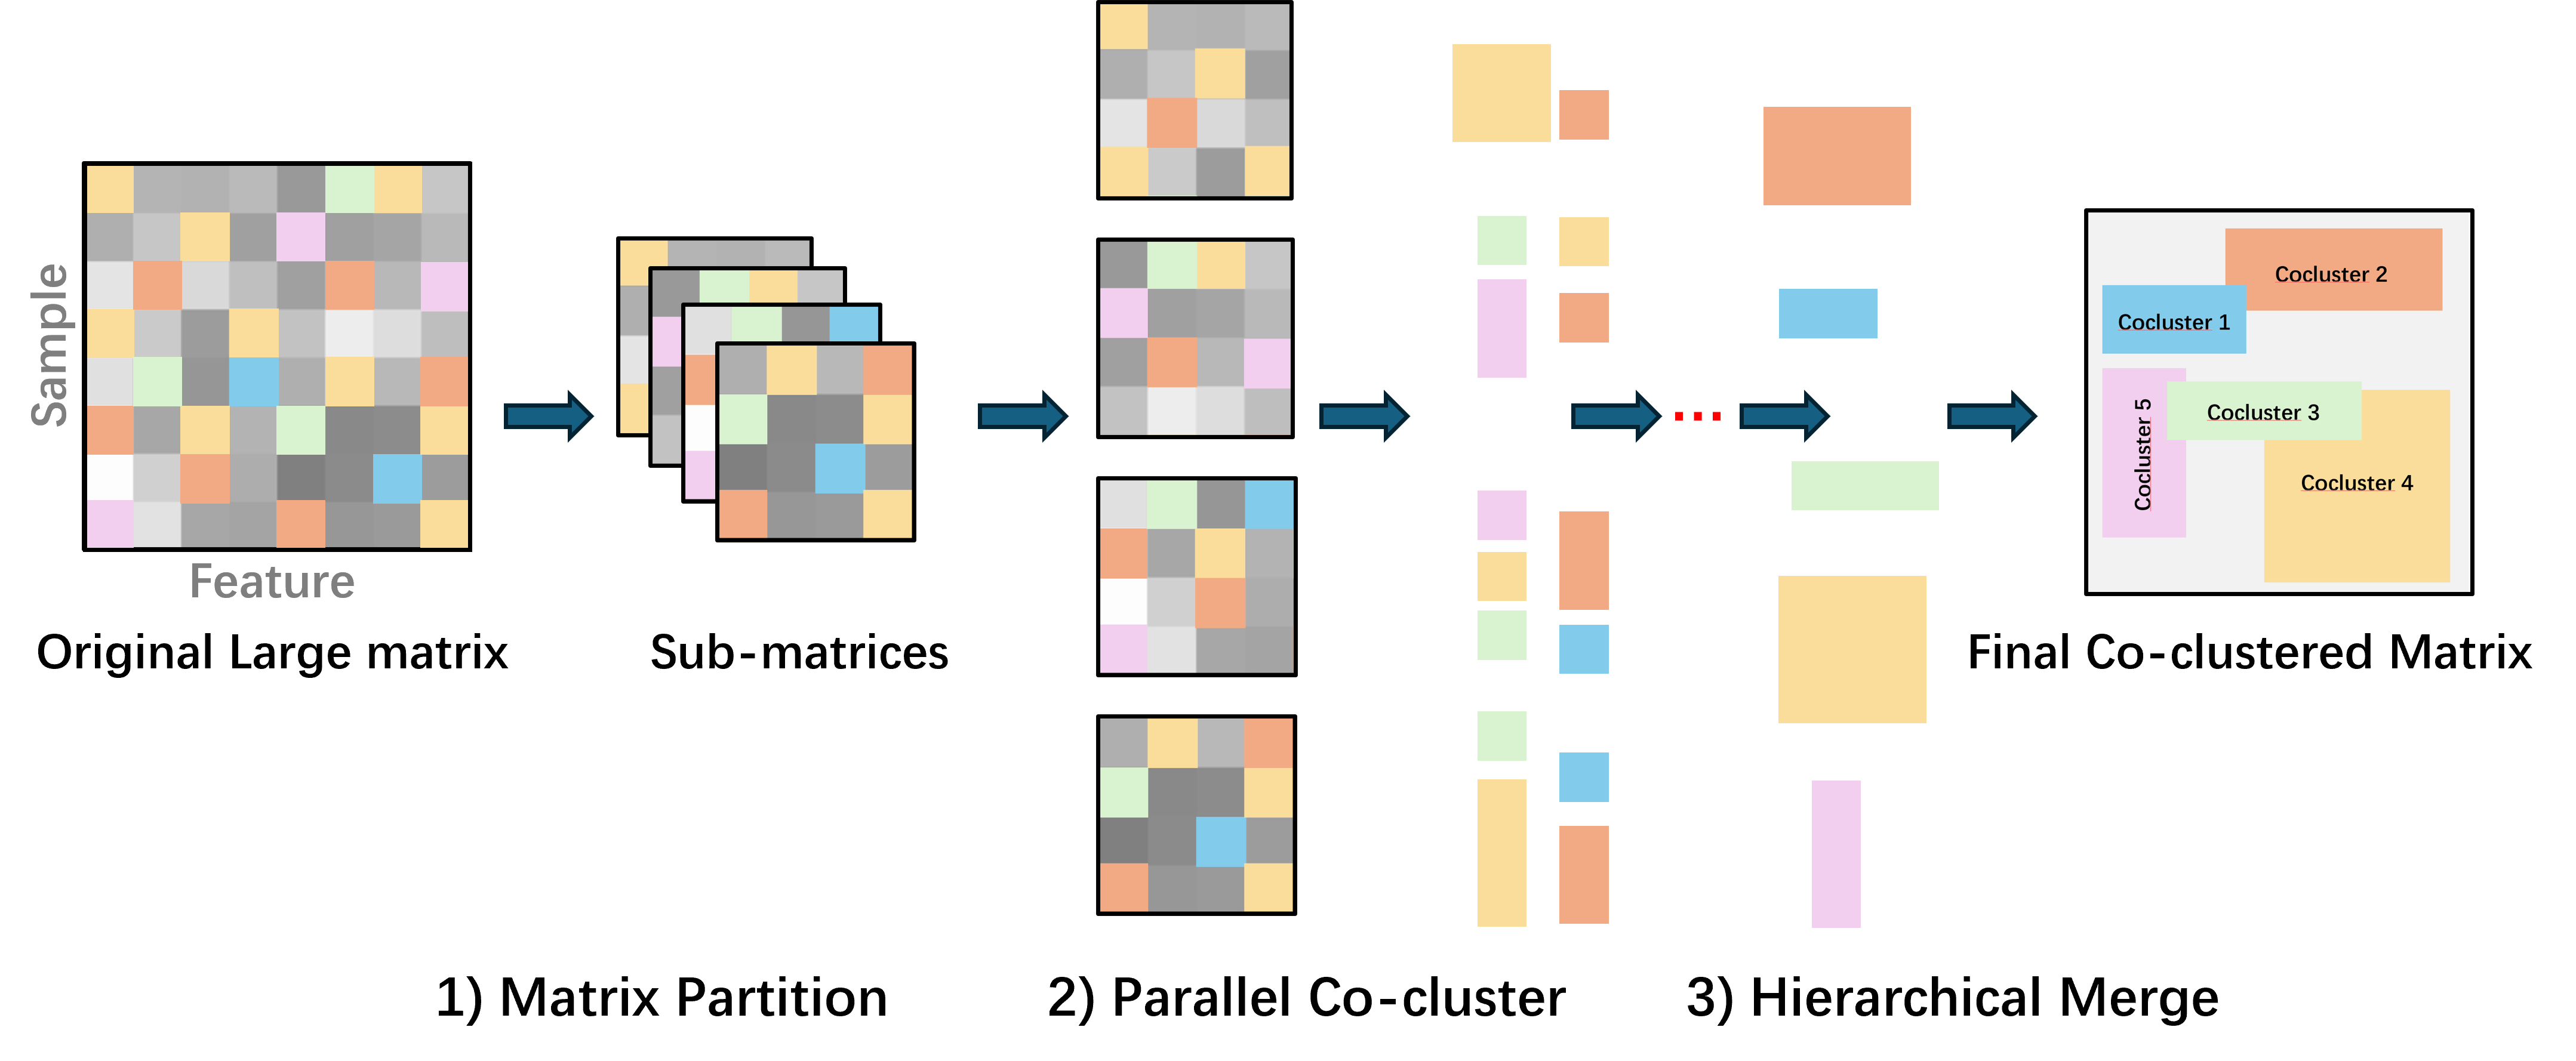
\includegraphics[width=0.8\linewidth]{workflow.png}
    \caption{Workflow of our proposed scalable co-clustering method for large matrices.}
    \label{fig:workflow}
\end{figure*}
This paper presents a novel and scalable co-cluster method specifically designed for large matrices, as shown in \Cref{fig:workflow}. This method applies a probabilistic model-based optimal partitioning algorithm, which not only predicts the ideal number and sequence of partitions for maximizing computational efficiency but also ensures the effectiveness of the co-clustering process.

Our method involves partitioning large matrices into smaller, manageable submatrices. This strategic partitioning is meticulously guided by our algorithm to facilitate parallel processing. By transforming the computationally intensive task of co-clustering a large matrix into smaller, parallel tasks, our approach significantly reduces computational overhead and enhances scalability.

Following the partitioning, each submatrix undergoes a co-clustering process. This is implemented via the application of Singular Value Decomposition (SVD) and $k$-means clustering on the resulting singular vectors. This pivotal step ensures the adaptability of our method, allowing our algorithm to tailor its approach to the unique characteristics of each submatrix, thus optimizing clustering results.

Furthermore, our method integrates a novel hierarchical merging strategy that combines the co-clustering results from all submatrices. This integration provides more fine-grained insight into each submatrix and enhances the overall accuracy and reliability of the co-clustering results. Our method, validated and optimized through a comprehensive process, showed efficiency in handling large-scale datasets that were never reached before.


\subsection{Large Matrix Partitioning}
% Description of the matrix partitioning process and criteria for partitioning.
The primary challenge in co-clustering large matrices is the risk of losing meaningful co-cluster relationships when the matrix is partitioned into smaller submatrices. To address this, we introduce an optimal partitioning algorithm underpinned by a probabilistic model. This model is meticulously designed to navigate the complexities of partitioning, ensuring that the integrity of co-clusters is maintained even as the matrix is divided. The objective of this algorithm is twofold: to determine the optimal partitioning strategy that minimizes the risk of fragmenting significant co-clusters and to define the appropriate number of repartitioning iterations needed to achieve a desired success rate of co-cluster identification.

\subsubsection{Partitioning and Repartitioning Strategy based on the Probabilistic Model}
Our probabilistic model serves as the cornerstone of the partitioning algorithm. It evaluates potential partitioning schemes based on their ability to preserve meaningful co-cluster structures within smaller submatrices. The model operates under the premise that each atom-co-cluster (the smallest identifiable co-cluster within a submatrix) can be identified with a probability $p$. This probabilistic model allows us to estimate the likelihood of successfully identifying all relevant co-clusters across the partitioned submatrices.

In the scenario where the matrix $A$ is partitioned into $m \times n$ blocks, each block has size $\phi_i \times \psi_j$, that is, $M=\sum_{i=1}^m \phi_i$ and $N=\sum_{j=1}^n \psi_j$, the joint probability of $M_{(i,j)}^{(k)}$ and $N_{(i,j)}^{(k)}$ are
\begin{equation}
    \label{eq:joint_probability}
    \begin{split}
        P(M_{(i,j)}^{(k)} & < T_m, N_{(i,j)}^{(k)} < T_n)                                                                           \\
                          & = \sum_{\alpha=1}^{T_m-1} \sum_{\beta=1}^{T_n-1} P(M_{(i,j)}^{(k)} = \alpha) P(N_{(i,j)}^{(k)} = \beta) \\
                          & \le \exp[-2 (s_i^{(k)})^2 \phi_i + -2 (t_j^{(k)})^2 \psi_j]
    \end{split}
\end{equation}
where $s_i^{(k)}$ and $t_j^{(k)}$ are the minimum row and column sizes of co-cluster $C_k$ in block $B_{(i,j)}$, the size of the co-cluster $C_k$ is $M^{(k)} \times N^{(k)}$, and $M^{(k)}$ and $N^{(k)}$ are the row and column sizes of co-cluster $C_k$, respectively.

% the size of co-cluster Ck∈RM(k)×N(k)C_k \in \mathbb{R}^{M^{(k)} \times N^{(k)}} that falls into block B(i,j)B_{(i,j)} is M(k)(i,j)×N(k)(i,j)M_{(i,j)}^{(k)} \times N_{(i,j)}^{(k)};

Thus, the probability of identifying all co-clusters is given by

\begin{equation}
    \begin{split}
        P(\omega_k) & \le \exp \left\{ -2 [\phi m (s^{(k)})^2 + \psi n (t^{(k)})^2] \right\},
    \end{split}
\end{equation}
and
\begin{equation}
    \begin{split}
        P & = 1 - P(\omega_k)^{T_p}                                                                                                       \\
          & \ge 1 - \exp \left\{ -2 T_p [\phi m (s^{(k)})^2 + \psi n (t^{(k)})^2] \right\} \label{eq:prob_of_identifying_all_co_clusters}
    \end{split}
\end{equation}
where $P(\omega_k)$ is the probability of the failure of identifying co-cluster $C_k$, $T_p$ is the number of sampling times, $\phi$ and $\psi$ are the row and column block sizes, and $s^{(k)}$ and $t^{(k)}$ are the minimum row and column sizes of co-cluster $C_k$.

\Cref{eq:prob_of_identifying_all_co_clusters} is central to our algorithm for partitioning large matrices, providing a probabilistic model to optimize our strategy and preserve co-cluster integrity. It quantifies the likelihood of identifying all relevant co-clusters within partitioned blocks, helping mitigate risks of fragmentation.

Using \eqref{eq:prob_of_identifying_all_co_clusters}, we can establish a constraint between the repartitioning time $T_r$ and the partition solution $Part$, ensuring adherence to a predetermined success rate and minimizing the risk of co-cluster fragmentation. Details of these constraints are discussed in the appendix due to space limitations.

\subsubsection{Optimization and Computational Efficiency}
Optimizing the partitioning process for computational efficiency is crucial in both academic and industrial applications. Our optimization strategy focuses on minimizing running time without compromising the integrity of co-cluster identification.

We assess various partitioning configurations to balance computational resource allocation and success rate adherence. By evaluating the impact of different schemes, we identify strategies that meet co-clustering criteria and optimize resource use.

To ensure efficiency without sacrificing quality, we introduce conditions for optimization that maintain co-cluster identification success. These conditions provide a mathematical basis for balancing computational efficiency and co-cluster identification fidelity.

The optimization must satisfy:
\begin{equation}
    \label{eq:optimization_condition}
    T_p = \text{argmin}_{T_p} \{
    1 - \exp \{ -2 T_p [\phi m (s^{(k)})^2 + n (t^{(k)})^2] \} \ge P_{\text{thresh}} \}
\end{equation}

Adhering to these conditions ensures our optimization efforts preserve the effectiveness of co-cluster discovery, making the partitioning algorithm fast, efficient, and robust across various datasets and challenges.

\subsection{Co-clustering on Small Submatrices}
% Detailed method for co-clustering within each of the submatrices.

\subsubsection{Atom-co-clustering Algorithm}
Our framework, which encompasses both partitioning and ensembling, offers remarkable flexibility, allowing it to be compatible with a wide range of atom-co-clustering methods. For the sake of making this paper comprehensive and self-contained, we provide an introduction to the atom-co-cluster method herein. The only requirement for an atom-co-clustering method to be compatible with our framework is that it must be able to identify co-clusters under a given criterion with a probability $p$, or more relaxed conditions, has a lower bound estimate of the probability of identifying co-clusters equipped with a validation mechanism.

\subsubsection{Atom-co-clustering Algorithm}
Our framework's flexibility allows it to be compatible with various atom-co-clustering methods. For an atom-co-clustering method to integrate with our framework, it must identify co-clusters under a given criterion with a certain probability $p$ or provide a lower bound estimate of this probability with a validation mechanism.

\subsubsection{Graph-based Spectral Co-clustering Algorithm}
Spectral co-clustering (SCC) is widely used for high-dimensional data due to its effectiveness in partitioning data into clusters based on graph Laplacian eigenvectors \cite{vonluxburg2007TutorialSpectralClustering}. SCC constructs a bipartite graph $G=(U,V,E)$ from the data matrix $A$, where $U$ and $V$ represent rows and columns, respectively, and $E$ are weighted edges indicating relationships.

The Laplacian matrix $L = D - W$ is computed, where $D$ is the degree matrix, and $W$ is the weighted adjacency matrix. Eigenvectors of the smallest positive eigenvalues of $L$ are used to partition the graph. The normalized matrix $A_n = D^{-1/2} A D^{-1/2}$ is factorized using singular value decomposition (SVD), and the resulting singular vectors are used for clustering.

For co-clustering, we apply $k$-means to the rows of the matrix formed by stacking the left and right singular vectors of $A_n$. This method effectively identifies clusters in high-dimensional data, making it suitable for our framework \cite{dhillon2001CoclusteringDocumentsWords}.

\subsection{Hierarchical Co-cluster Merging}
% Explanation of how co-clustered results from submatrices are aggregated.

Hierarchical co-cluster merging is a novel approach that combines the results of co-clustering on submatrices to produce a final co-clustered result.
The merging method is designed to enhance the accuracy and robustness of the co-clustering outcome by leveraging the design of the partitioning algorithm. The hierarchical merging process iteratively combines the co-clusters from each submatrix, ensuring that the final co-clustered result is comprehensive and consistent across all submatrices. This iterative merging process is crucial for addressing issues of heterogeneity and model uncertainty, ensuring that the final co-clustering results are reliable and robust.

\subsection{Algorithmic Description}
% Step-by-step algorithmic description of the process in pseudocode.
Our proposed  Optimal Matrix Partition and Hierarchical Co-cluster Merging Method is outlined in Algorithm \ref{alg:method}. The algorithm
is an advanced algorithm designed for efficient co-clustering of large data matrices. The algorithm begins by initializing a block set based on predetermined block sizes. For each co-cluster in the given set, the algorithm calculates specific values $s^{(k)}$ and $t^{(k)}$, which are then used to determine the probability $P(\omega_k)$ of each co-cluster. If this probability falls below a predefined threshold $P_{\text{thresh}}$, the algorithm partitions the data matrix $A$ into blocks $B$ and performs co-clustering on these blocks. This step is crucial for managing large datasets by breaking them down into smaller, more manageable units. After co-clustering, the results from each block are aggregated to form the final co-clustered result $\mathcal{C}$. The algorithm's design allows for a flexible and efficient approach to co-clustering, particularly suited to datasets with high dimensionality and complexity.

\begin{algorithm}[!t]
    \caption{Optimal Matrix Partition and Hierarchical Co-cluster Merging Method}\label{alg:method}
    \begin{algorithmic}[1]
        \REQUIRE{Data matrix $A \in \mathbb{R}^{M \times N}$, Co-cluster set $C = \{C_k\}_{k=1}^K$, Block sizes $\{\phi_i\}_{i=1}^m$, $\{\psi_j\}_{j=1}^n$, Thresholds $T_m$, $T_n$, Sampling times $T_p$, Probability threshold $P_\text{thresh}$;}
        \ENSURE{Co-clustered result $\mathcal{C}$;}
        \STATE Initialize block set $B = \{B_{(i,j)}\}_{i=1}^m,_{j=1}^n$ on $\phi_i$ and $\psi_j$
        \STATE Calculate $s^{(k)}$ and $t^{(k)}$ for each co-cluster $C_k$
        \FOR{$k=1$ to $K$}
        \STATE Calculate $P(\omega_k)$ for co-cluster $C_k$
        \IF{$P(\omega_k) < P_{thresh}$}
        \STATE Partition matrix $A$ into blocks $B$ and perform co-clustering
        \STATE Aggregate co-clustered results from each block
        \ENDIF
        \ENDFOR
        \RETURN Aggregated co-clustered result $\mathcal{C}$
    \end{algorithmic}
\end{algorithm}


\begin{table}[b]
	\caption{Sample table title}
	\centering
	\begin{tabular}{lll}
		\toprule
		\multicolumn{2}{c}{Part}                   \\
		\cmidrule(r){1-2}
		Name     & Description     & Size ($\mu$m) \\
		\midrule
		Dendrite & Input terminal  & $\sim$100     \\
		Axon     & Output terminal & $\sim$10      \\
		Soma     & Cell body       & up to $10^6$  \\
		\bottomrule
	\end{tabular}
	\label{tab:table}
\end{table}

\printbibliography

\end{document}
